\subsection{The material, $\beta$-Ga$_2$O$_3$}

The primitive unit cell of $\beta$-Ga$_2$O$_3$ is base-centered monoclinic. The structure has three inequivalent oxygen sites and two inequivalent gallium sites. The unit cell is shown in Figure \ref{fig:unit_cell}. The oxygen sites are named O(I), (OII) and O(III). O(I) and O(II) are threefold coordinated, while O(III) is fourfold coordinated (Figure \ref{fig:oxygen_sites}). The gallium sites are called Ga(I) and Ga(II). Ga(I) and Ga(II) are tetrahedrally and octahedrally coordinated, respectively \cite{dft_ga2o3}. Figure \ref{fig:gallium_sites} shows the different sites in the super cell. 

\begin{figure}[H]
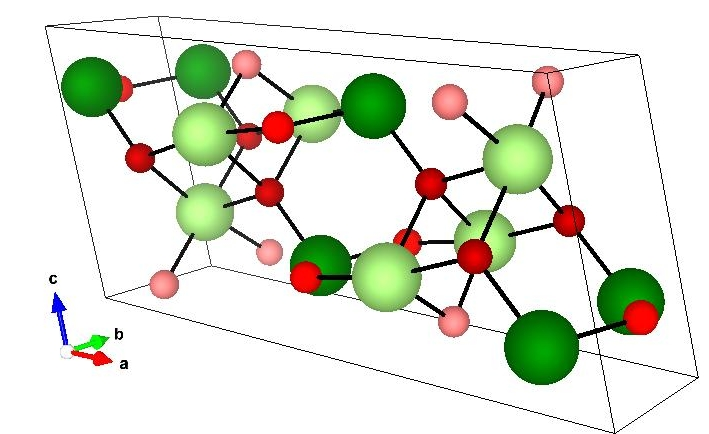
\includegraphics[width=\linewidth]{../fig/unitcell}\caption{This figure shows the primitive unit cell of $\beta$-Ga$_2$O$_3$.}\label{fig:unit_cell}
\end{figure}

\begin{figure}[H]
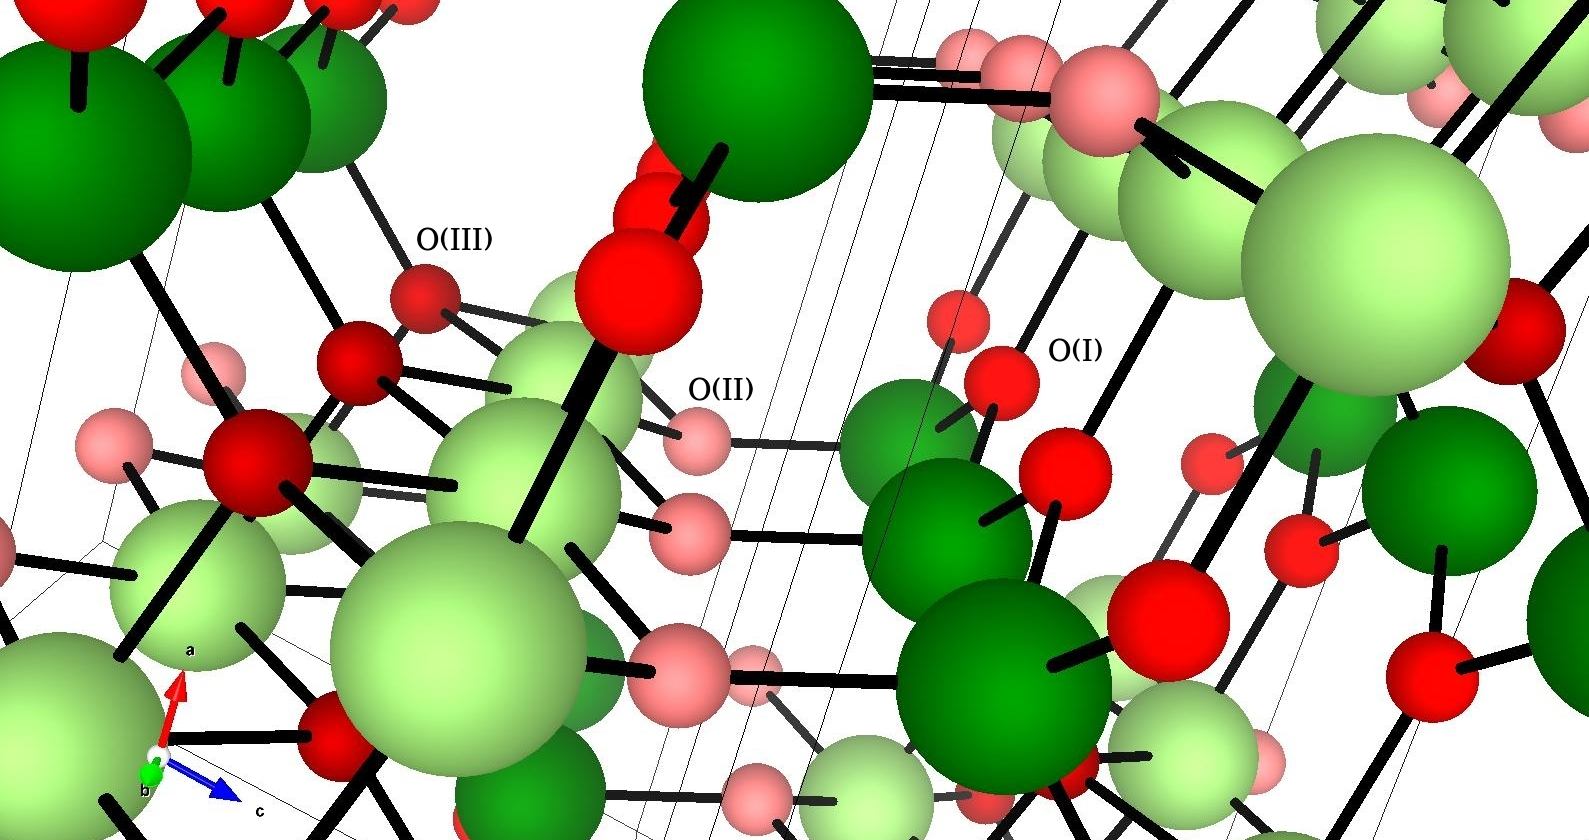
\includegraphics[width=\linewidth]{../fig/Ga2O3-different-sites-names}\caption{This figure shows the inequivalent oxygens in the unit cell. There are three different oxygen sites, they are color coded and named.}\label{fig:oxygen_sites}
\end{figure}

\begin{figure}[H]
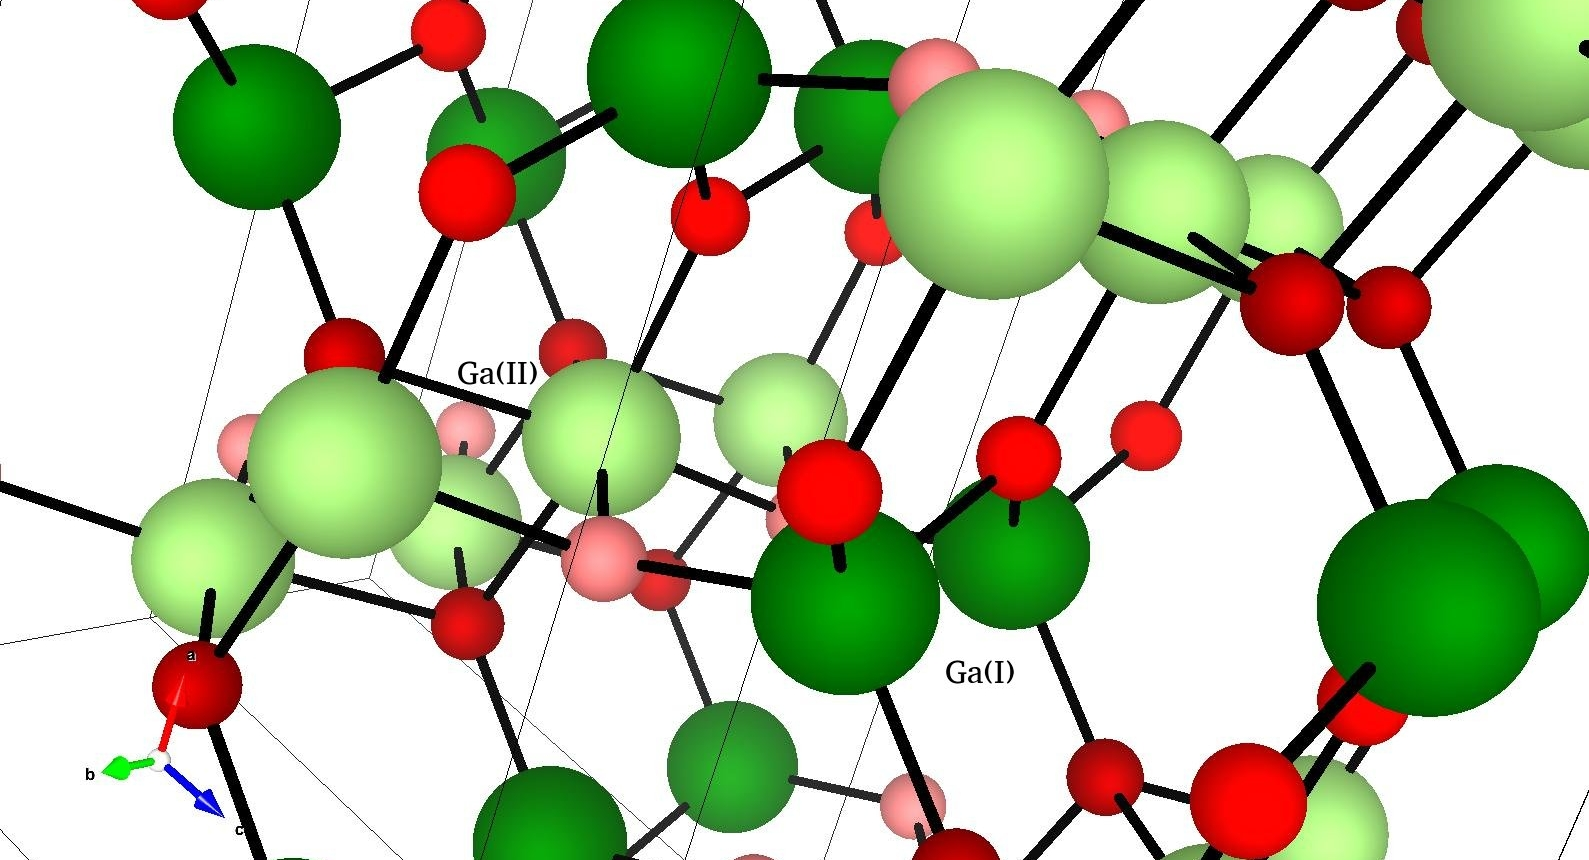
\includegraphics[width=\linewidth]{../fig/Ga2O3-Ga-sites}\caption{This figure shows the inequivalent gallium sites in the unit cell.}\label{fig:gallium_sites}
\end{figure}


\begin{figure}[H]
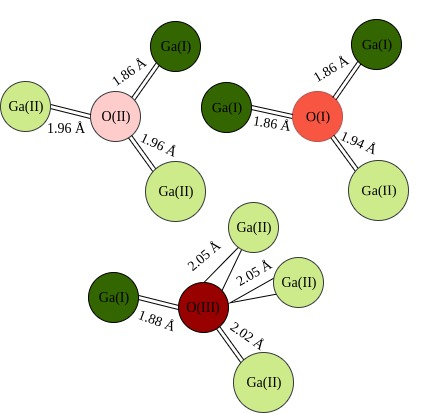
\includegraphics[width=\linewidth]{../fig/distances}\caption{This figure shows the distances at the diffrent oxygen sites of in the relaxed super cell. We assume that the distances are similar for all equivalent sites in the supercell.}\label{fig:distances}
\end{figure}

\subsection{DFT Convergence}

\textit{Should I write some on the 'theory' of DFT convergence?}

What do energy cut off represent and what does the k-point density represent?

Balance between CPU time and accuracy in results.

\subsection{DFT Formation Energy}

\textit{Should I write something on how to compare energies?}

Write about oxygen molecule (difference in INCAR). Assumptions about o-rich conditions.

\[
E_f = E_b - E_v - \mu_O
\]